\documentclass[conference]{IEEEtran}
\IEEEoverridecommandlockouts

% Packages
\usepackage{cite}
\usepackage{amsmath,amsfonts}
\usepackage{algorithm}
\usepackage{algpseudocode}
\usepackage{graphicx}
\usepackage{textcomp}
\usepackage{xcolor}
\usepackage{booktabs}
\usepackage{adjustbox}
\usepackage{listings}

\usepackage{verbatim}
\usepackage{multirow}

\usepackage{subcaption}

%\def\BibTeX{{\rm B\kern-.05em{\sc i\kern-.025em b}\kern-.08em
    %T\kern-.1667em\lower.7ex\hbox{E}\kern-.125emX}}

\begin{document}

\author{}
\title{Deliverable report 2\\
\footnotesize \textit{"Diego Oniarti": Mat: 257835, \texttt{diego.oniarti@studenti.unitn.it}, GitRepo: \texttt{https://github.com/diego-oniarti/GPU-Computing-2025-257835}}}

\maketitle

\begin{abstract}
% [max 200 words]\\
% The sparse matrix-dense vector multiplication (SpMV) is a common linear algebra operation involving a sparse matrix and a dense vector. SpMV is widely used in many real-world applications such as \dots
% 
% This deliverable discusses \dots
    This deliverable proposes improvements on the implementation shown in the previous one.\\
    Two different implementations will be shown, the first simply addressing the more glaring issues of the old kernel through the use of shuffle operations and other CUDA features. The second one will rely heavily on shared memory to increase the kernel performance on structured matrices with higher local density of non-zeros.
\end{abstract}

\begin{IEEEkeywords}
Sparse Matrix, SpMV, CUDA, Parallelization, Storage Format, Shared Memory, Shuffle Operation
\end{IEEEkeywords}

\section{Introduction}
% [max 300 words]\\
The implementation proposed in the previous deliverable mapped each row of the matrix to a single warp. The threads in each warp then iterated through the row with a stride equal to the warp size to guarantee coalesced memory access to some of the data structures in used. However, due to the indirect access to the vector $x$ used in the multiplication, many of the accesses were not coalesced. The solutions in this deliverable will try to attenuate this problem to improve performance.

The results will be compared with the ones from the previous work, as well as the state of the art solutions to the SpMV problem.

\section{Problem Statement}
% Define the problem statement, including a description of the storage format used and a brief discussion of the parallelization approach (e.g., using CUDA).
% \subsection{Storage Format}
% Details about the format (e.g., CSR, COO, etc.) \dots
% 
% \subsection{Parallelization}
% Describe the CUDA implementation approach \dots
The two main CUDA features that are gonna be explored in this deliverable are shuffle operations and shared memory, but some other smaller optimization will be used as well.

\subsection{Shared Memory}
Shared memory is a region of memory present on the GPU which can be accessed with latency orders of magnitude lower than global memory. This makes shared memory a perfect instrument to build user-defined caches (the use we're going to make of it), since data can be loaded from global memory once into shared and then more quickly be accessed from there.

The two main drawbacks of shared memory are the size and bank conflicts. The first is an issue because the size of shared memory is relatively small, forcing the developer to decide which bits of data are worth transferring to shared memory and which ones are not.\\
Shared memory is divided into banks which can be accessed simultaneously by different threads. If more threads try to access the same bank however (a conflict), the operations get serialized, lowering the effective throughput. It is important to avoid this scenario whenever possible. \cite{sharedMem}

\subsection{Shuffle Operations}
Warp shuffle functions are used to exchange and share variables between threads within the same warp.\\
This allows for single variables to be exchanged simultaneously for all threads without relying on shared or global memory. \cite{shuffleOps}

% \section{State of the Art}
% Describe the available library solutions for the SpMV problem, including references and citations.

\section{Methodology and Contributions}

% Describe the methodology used during the analysis, the compared algorithms and the expected outcomes. Use pseudo-codes like Algorithm \ref{alg:COOaggr} to describe your own implemented kernels.
% 
% \noindent Include at least the following implementations:
% \begin{itemize}
%     \item Naive CPU implementation
%     \item Optimised CPU implementation based on cache behaviour
%     \item GPU naive implementation
% \end{itemize}
% 
% \noindent For the analysis include
% \begin{itemize}
%     \item Valgrind and runtime comparison between the CPU implementations 
%     \item Runtime CPU vs GPU comparison looping over different matrix dimensions
% \end{itemize}
% 
% \begin{algorithm}[ht!]
% \caption{Algorithm for the vector addition}
% \algorithmicrequire~The input vectors $a$ and $b$ of size $nnz$.
% \begin{algorithmic}[1]
% \Procedure{Function}{$a$, $b$, $nnz$}
% \State $c \gets \emptyset$
% \For{$i$ in $\{1 \dots nnz\}$ \textbf{parallel}}
% \State $c[i] = a[i] + b[i]$
% \EndFor
% \State \textbf{return} $c$\Comment{the result vector}
% \EndProcedure
% \end{algorithmic}
% \label{alg:COOaggr}
% \end{algorithm}

In this section I'm going to briefly present the best implementation from the previous deliverable (warp-per-row), with its strengths and weaknesses. This is gonna be followed by an improved version that makes minimal changes and uses the shuffle functions to improve performance. The third version of the kernel will be a further improvement based on shared memory.

\subsection{warp-per-row}
\begin{algorithm}[ht!]
    \caption{warp-per-row}
    \begin{algorithmic}[1]
        \Procedure{Kernel}{$vals$, $xs$, $ys$, $vec$, $nnz$, $nrows$, $result$, $buffer$}
        \State $id \gets block\_id \cdot block\_dim + thread\_id$
        \State $wid \gets thread\_id / warp\_size$
        \State $lane \gets thread\_id \% warp\_size$
        \State $row \gets block\_id \cdot block\_size / warp\_size + wid$

        \State $buffer[tid] \gets 0$ \Comment{Always initiated to $0$ for safety}
        \If {$row<nrows$}
        \State $start \gets ys[row]$
        \State $end\gets ys[row+1]$
        \State $sum \gets 0$
        \State //Iterate through the assigned row
        \For {$i=start+lane;\ i<end;\ i+=32$}
        \State $sum += vals[i]\cdot vec[xs[i]]$
        \EndFor
        \State $buffer[id] \gets sum$
        \EndIf
        \State // Reduction
        \For {$s=1;\ s<warp\_size; s=s^2$}
        \State \_\_syncthreads()
        \If {$id\&(s^2-1) == 0$}
        \State $buffer[tid] += buffer[tid+s]$
        \EndIf
        \EndFor
        \If {$lane==0 \wedge row<nrows$}
            \State $ret[row] \gets buffer[id]$
        \EndIf
        \EndProcedure
    \end{algorithmic}
    \label{algo:warprow}
\end{algorithm}
In this implementation we have a whole warp (32 threads in this case) working on each row of the matrix. Each thread calculates the partial sum of the elements that are assigned to it and stores it in a common buffer. A reduction of the elements in the buffer is then performed cooperatively by all the threads in the warp. Finally the thread with the lowest id moves the total sum in the result vector.

The access to the $vals$ and $xs$ vectors is coalesced thanks to the stride being equal to the warp size, but the indirect access to the dense vector is not, tanking performance.

The reduction used to sum the partial results is performed cooperatively, making it faster than a linear scan through the buffer, but it still requires repeated access to a global memory buffer, which has high latency.

\subsection{Improved}
\begin{algorithm}[ht!]
    \caption{improved}
    \begin{algorithmic}[1]
        \Procedure{Kernel}{$vals$, $xs$, $ys$, $vec$, $nrows$, $result$}
        \State //Same variable initialization
        \If {$row\geq rows$} \Comment{Early return}
        \State \Return
        \EndIf
        \State $start \gets ys[row]$
        \State $end \gets ys[row+1]$
        \State $sum = 0$
        \For {$i=start+lane;\ i<end;\ i+=32$}
        \State $sum += vals[i] \cdot \_\_ldg(\&vec[xs[i]])$
        \EndFor
        \State //Reduction
        \For {$off = 16;\ off>0;\ off=\sqrt{off}$}
        \State $mask\gets0xffffffff$
        \State $sum += \_\_shfl\_down\_sync(mask, sum, off)$
        \EndFor
        \If {$lane==0$}
            \State $ret[row] \gets buffer[id]$
        \EndIf
        \EndProcedure
    \end{algorithmic}
    \label{algo:improved}
\end{algorithm}
% TODO Nomina __restrict__, __ldg, shuffle al posto di buffer


\section{System Description and Experimental Set-up}
% Use this section to describe system, dataset and experimental set-up.
Each run has been performed with $3$ warm-up cycles and $10$ timed runs, which are then averaged. The timing of the CPU implementation was measured with the \texttt{gettimeofday} function from the standard library, while the GPU kernels were timed using CUDA events.

Additionally, the GPU kernels have been tested with different block sizes, ranging from 32 to 1024 and doubling each time.

\subsection{System Description}
% Describe the used system and the software environment (CUDA version, GCC version, \dots). Decide which information are valuable to group into a table like Table \ref{tab:system_description} and which are more valuable to be described in the text.

All the code has been ran on the Baldo cluster, with an AMD EPYC 9334 32-CORE Processor and a NVIDIA A30 GPU.\\
The CUDA version being used is 12.5.0 and the code has been compiled with NVCC 12.5.
The theoretical memory bandwidth for the GPU is around $933$GB/s.

\subsection{Dataset description}
Each of the algorithms was ran on 4 different kind of matrices, with different sizes, types of data, and levels of organization.\\
Three of the matrices have been taken from SuiteSparse Matrix Collection, while one is generated at runtime with a completely random distribution.
\begin{table}[ht!]
    \centering
    \begin{adjustbox}{width=\columnwidth}
        \begin{tabular}{l|r|r|rl|l}
            name & rows & columns & nonzeros & (\%) & type \\
            \hline
            lp\_ganges\footnote & 1309 & 1706 & 6937 & 0.3106\% & real \\
            delaunay\_n23\footnotemark & 8388608 & 8388608 & 50331568 & 7.152546e-5\% & binary \\
            Stanford\_Berkeley\footnotemark & 683446 & 683446 & 7583376 & 0.001624\% & binary \\
            random & 30000 & 20000 & 6001585 & 1.000264\% & real \\
        \end{tabular}
    \end{adjustbox}
    \caption{Test matrices}
    \label{tab:matrices}
\end{table}
\footnotetext[1]{https://www.cise.ufl.edu/research/sparse/matrices/LPnetlib/lp\_ganges}
\footnotetext[2]{https://www.cise.ufl.edu/research/sparse/matrices/DIMACS10/delaunay\_n23}
\footnotetext[3]{https://www.cise.ufl.edu/research/sparse/matrices/Kamvar/Stanford\_Berkeley}

\begin{figure}
    \centering
    \begin{subfigure}[b]{0.45\linewidth}
        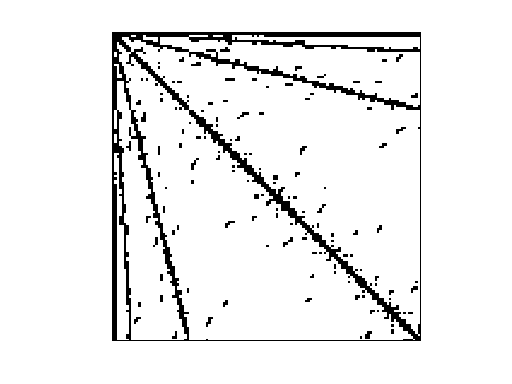
\includegraphics[width=\linewidth]{images/delaunay_n23.png}
        \caption{Delaunay Graph}
        \label{fig:delaunay_n23}
    \end{subfigure}
    \hfill
    \begin{subfigure}[b]{0.45\linewidth}
        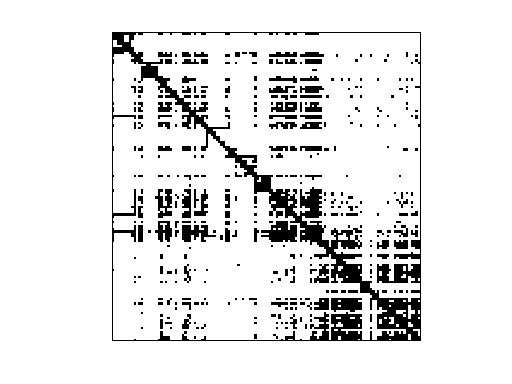
\includegraphics[width=\linewidth]{images/Stanford_Berkeley.png}
        \caption{Stanford-Berkeley Dataset}
        \label{fig:stanford_berkeley}
    \end{subfigure}
    \vspace{0.5cm}
    \begin{subfigure}[b]{0.45\linewidth}
        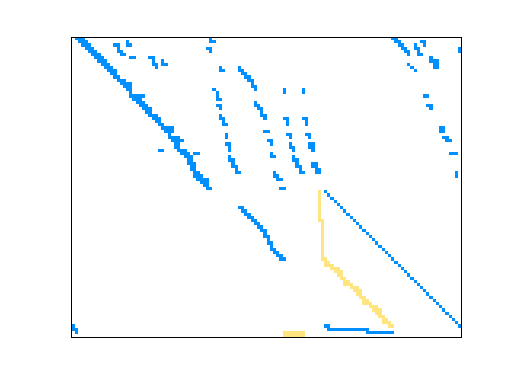
\includegraphics[width=\linewidth]{images/lp_ganges.png}
        \caption{LP-Ganges Dataset}
        \label{fig:lp_ganges}
    \end{subfigure}
    
    \caption{Datasets distributions}
    \label{fig:Dataset-images}
\end{figure}

\section{Experimental Results}
% Present and discuss results. Include plots and tables when required (like Figure \ref{fig:enter-label}). Do not simply describe the figures; criticise the achieved results by underlining how they confirm/differ from the expected outcomes described in Section \ref{sec:methodology}.
% 
% \begin{figure}
%     \centering
%     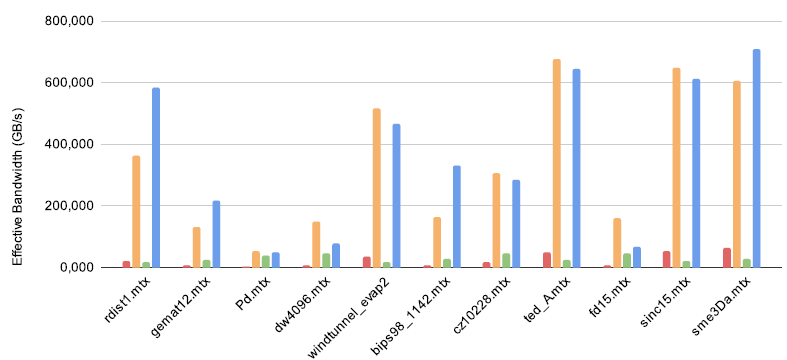
\includegraphics[width=0.95\linewidth]{SampleImage.png}
%     \caption{Caption}
%     \label{fig:enter-label}
% \end{figure}

The results immediately show that my assumptions on the chunked CPU implementation were wrong. Each run of that algorithm take up to double the time of the naive implementation on small matrices, and goes past the 5 minutes of allotted time on larger matrices.\\
The implementation aimed at taking advantage of temporal locality when reading the vector, sacrificing some of the spatial locality when reading the matrix. This trade-off, combined with the added complexity in iterating over the rows multiple times and handling the \textit{row\_counters} vector, has proven not to be worth it.

\begin{table}[ht!]
    \centering
    \begin{adjustbox}{width=\columnwidth}
        \begin{tabular}{l|ccc|ccc|ccc|ccc}
            \toprule
& \multicolumn{3}{c}{Delaunay} & \multicolumn{3}{c}{LP\_Ganges} & \multicolumn{3}{c}{stanford} & \multicolumn{3}{c}{random} \\
\cmidrule(lr){2-4} \cmidrule(lr){5-7} \cmidrule(lr){8-10} \cmidrule(lr){11-13}
& CPU & thread & warp & CPU & thread & warp & CPU & thread & warp & CPU & thread & warp \\
\midrule
            threads per block & - & 256 & 128 & - & 1024 & 128 & - & 64 & 128 & - & 1024 & 64 \\
            mean time (ms) & 185.34 & 0.466 & 8.013 & 26.7 & 0.016 & 0.012 & 29 & 5.202 & 0.959 & 19.586 & 0.447 & 0.104 \\
            deviation (ms) & 2.288 & 0.001 & 0.003 & 1.567 & 0 & 0.001 & 0.065 & 0.249 & 0.017 & 0.017 & 0.001 & 0.001 \\
            bandwidth (GB/s) & 1.629 & 647.73 & 37.69 & 0.004 & 6.873 & 9.646 & 2.342 & 13.239 & 71.791 & 2.464 & 108 & 462.88 \\
            FLOPS & 271560 & 107955022 & 6280994 & 519 & 846801 & 1188493 & 515870 & 2915663 & 15810505 & 612323 & 26843502 & 115047352 \\
            \bottomrule
        \end{tabular}
    \end{adjustbox}
    \caption{Experimental results}
    \label{tab:results}
\end{table}
\textbf{Table \ref{tab:results}} shows the results of the three working algorithms on each dataset. The GPU implementations have been tested with different block sizes, but only the ones with the best results are shown.

The bandwidth of each algorithm, as shown in \textbf{Figure \ref{fig:chart}}, mostly follows a clear trend, with the increasing amount of parallelization leading to better performances. 

The only outlier in this trend is the Delaunay dataset, with the reason most likely being the first row of the graph. Looking at the distribution of the values in \textbf{Figure \ref{fig:delaunay_n23}}, it is visible that the first row of the graph is dense. This fact can possibly bring the second algorithm to take better advantage of the cache, beating the advantage that the third one would have had.

\begin{figure}
    \centering
    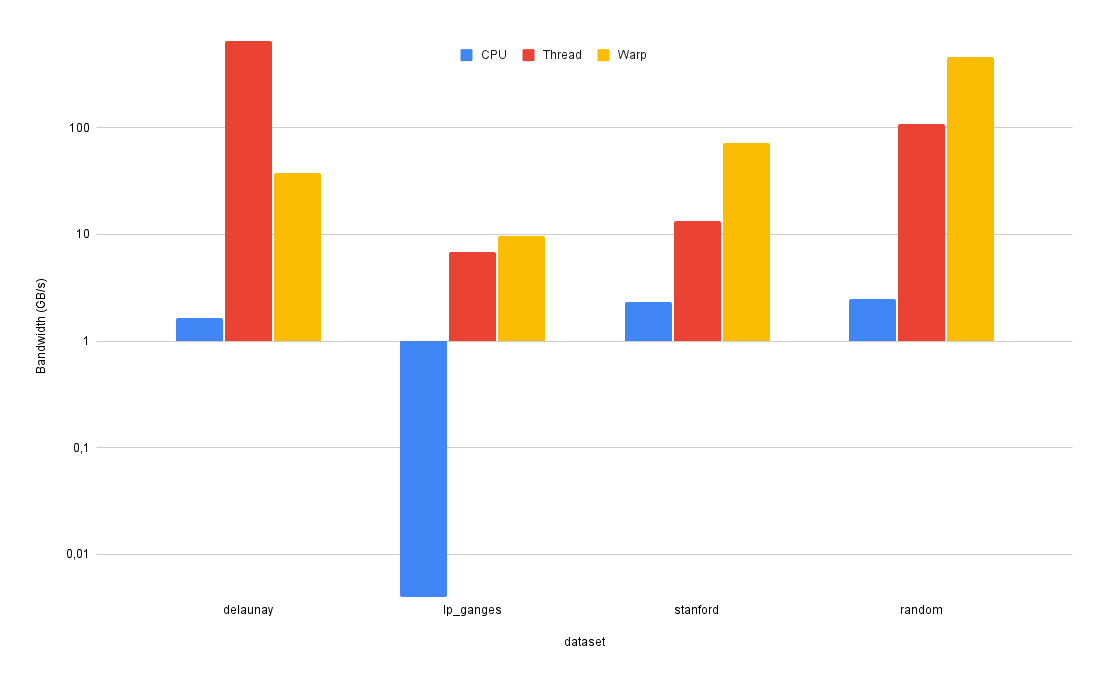
\includegraphics[width=0.95\linewidth]{images/chart.png}
    \caption{Bandwidths of the algorithms on the different datasets}
    \label{fig:chart}
\end{figure}

Lastly, \textit{cachegrind} has been used to measure the amount of cache misses. On the random matrix the naive CPU implementation gets 0.6\% D1 miss rate and 0.1\% LL miss rate. These results confirm that simply using the CSR format ensures a good usage of the cache.

\section{Conclusions}
% [max 200 words]\\
% Summarize findings and future work \dots
The use of the CSR format to store the matrix in memory has proven to be a useful tool to optimize the SpMV operation. The ordering of the elements based on their position in the matrix allows for a sequential access that is predictable and that can take good advantage of the cache.

Parallelization was shown to be orders of magnitude faster than the sequential operation on all datasets, with varying results on the kind of parallelization that yield the better performance.

Lastly, the attempt to find a better memory access pattern was unsuccessful. The trade-offs made when using the chunk based approach were likely too disadvantageous to bring any improvement.

\subsection{Future works}
As discussed earlier, there is a trend of improvement when moving from the first GPU implementation to the second one, with the exception of the results taken on the Delaunay Graph dataset. Further testing on different kinds of matrices could help determine whether this was a one-of occurrence or a common one.

Another improvement would be to use more threads for each row of the matrix being processed. This can however complicate the synchronization between threads if the implementation is not well thought out

Lastly, the use of global memory to store the buffer with the partial results of operations is an obvious slowdown. Future implementations would use shared memory and a better reduction algorithm to add together the partial sums.

\bibliographystyle{IEEEtran}
\bibliography{references}

\end{document}



% Deliverable 2
% Abstract
% Keep the introduction about the SpMV.
% Mention the previous deliverable
% State how this deliverable is gonna try and improve the results of the first.
% Also state there is gonna be a comparison with the state of the art solutions.
% 
%   I.    Introduction
% Explain which optimization have been made in the first deliverable and give an hint on which ones will be used in this one.
% 
%  II.    Problem Statement
% Better describe what shared memory and thread-communication operations are, and how they are gonna be used.
% 
% III.    Methodology and Contributions
% Describe the old version of the algorithm, the two improvements and their motivations.
% Describe the state of the art implementations.
% Describe the experimental setup?
% 
%  IV.    System Description and Experimental setup
% Same as the old one + the versions of the libraries used
% 
%   V.    Experimental results
% Comparison between old, shared, reduction, and both. (Hopefully the one using both will be the best)
% Compare the best result with the state of the art solutions
% 
%  VI.    Conclusions

